\documentclass[man,floatsintext,12pt,natbib]{apa6}
\usepackage[colorlinks=false]{hyperref}
\usepackage{amssymb}
\usepackage{amsmath}
\usepackage{graphicx}
\usepackage{grffile}
\usepackage{times}
\linespread{1.5}

\graphicspath{ {.resources/} }
\makeatletter
\def\maxwidth{\ifdim\Gin@nat@width>\linewidth\linewidth\else\Gin@nat@width\fi}
\def\maxheight{\ifdim\Gin@nat@height>\textheight\textheight\else\Gin@nat@height\fi}
\makeatother

% Scale images if necessary, so that they will not overflow the page margins by
% default, and it is still possible to overwrite the defaults using explicit
% options in \includegraphics[width, height, ...]{}
\setkeys{Gin}{width=\maxwidth,height=\maxheight,keepaspectratio}
\setlength{\parindent}{0pt} \setlength{\parskip}{6pt plus 2pt minus 1pt}
\setlength{\emergencystretch}{3em}  % prevent overfull lines
\providecommand{\tightlist}{%
\setlength{\itemsep}{0pt}\setlength{\parskip}{0pt}} \setcounter{secnumdepth}{0}

\begin{document}

\title{Linguistic Autobiography}
\shorttitle{Linguistic Autobiography}
\author{Edward Hern\'{a}ndez}
\date{2015-08-31}
\affiliation{College of William \& Mary}
\maketitle

\begin{figure}[htbp]
	\centering
	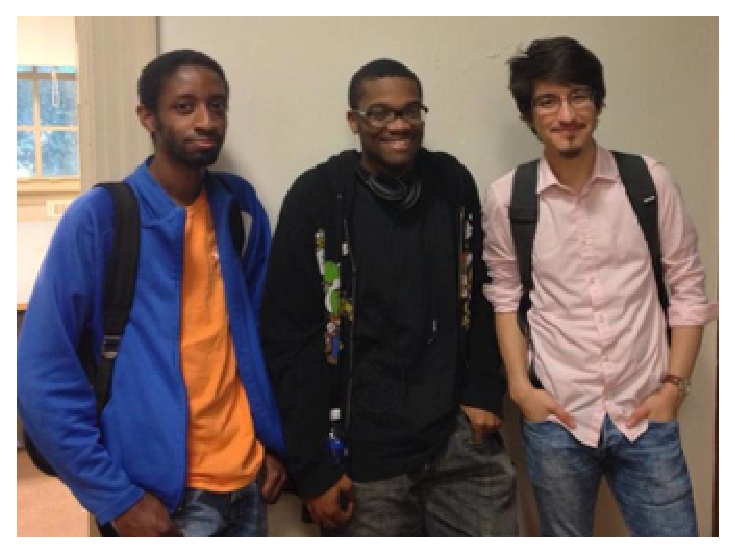
\includegraphics{ngare.clarke.hernandez}
\end{figure}

My name is Edward Hern\'{a}ndez. Here's a relatively old picture of me (with
Bishop and Jeffrey), but one of the best I've got, 
%it's a great photo!
since cameras and I don't tend to get along. I'm a junior majoring in
Linguistics. I am from Newport News, and until college, I hadn't lived anywhere
else. Despite not having moved around, I've been influenced by a few different
varieties of both English and Spanish.

Throughout my childhood, I was convinced that my mother's highly standardized
English was inherently good, and therefore better than my father's. My father
learned English as a second language late in elementary school, and he never
really learned the standard ways to conjugating verbs or choose pronouns. In
contrast, my mother's subjects and verbs always agreed and her pronouns always
took the correct case.  She kept The Little, Brown Handbook
\citep{RamseyFowler95} on a shelf in the living room next to the King James
Bible, and taught me to obey both.

Unfortunately, my father believed this standardization ideology as well.  It
caused him to be self-conscious about his nonstandard use of language. Despite
being fluent in Spanish, he refused to teach me any, or to even speak Spanish
around me. He was sure that since his variety of Spanish was bad, because it
was different from the high prestige varieties he held to be proper. He thought
that it would be a disservice to me to teach me anything but a standardized
variety. This meant that my Spanish education was left to my mother, a
non-native speaker who couldn't do anything but teach me dry, decades-old
Castilian out of a book. This, of course, did nothing but entrench
standardization ideology in my mind.

As a young child, I didn't question that this was correct. My ideas weren't
shaken at all until I started kindergarten. Suddenly I was surrounded by
classmates who spoke with a register that I had never been taught. I didn't
know, at the time, how to speak any way but formally, and I thought that the
fact that they didn't meant that they were ignorant. I hated it, and I disliked
them for it. Slowly, reluctantly, I approximated their registers to fit in. It
worked, but for years I felt guilty every time I produced a non-standardized
string. I knew that it was useful, but I thought of it as nothing more than a
necessary evil.

My ideology didn't change much until high school. I kept using the vernacular
I'd learned in school socially, but I hated it. I used my mother's standardized
English academically, and I felt good about that.  So did my teachers. I got
tons of praise for my writing. I was proud of my standardized English, but I
only used it academically, because I wanted to fit in. Then I found debate. It
was social, but my standardized English was perfect. It gave me a distinct
edge, since it made me sound professional and polished to the middle aged
college educated white judges. I was thrilled, and I made my debate language
progressively more standardized, arcane, and inaccessible. Eventually I found
myself spouting nonsense like:
\begin{quote}
	``Our alternative is queer unintelligibility: This is an enforced
	invisibility that resists the catachresis of the Symbolic that imposes
	identity on lack in a neurotic attempt to map out the blind spots in the
	social order.'' \citep[p.~19]{Pease11}
\end{quote}
% Good to bring up in class
I thought I was pretty great. Luckily, this didn't last all that long.  Another
debater, now a friend of mine, came along and crushed my debate case and my
language ideology in one fell swoop. Xe asserted that arcane English, like
mine, put up barriers to entry, hindering disabled persons, non-native and
non-standardized speakers of English from participating in debate. This was a
radically new idea for me, so I began to read everything I could find on the
topic. I finally stumbled on some critical theory that helped me through some
of my confusion, and that theory is what led me to consider studying
linguistics.

Now that I see the error of my ways, the dream is to eliminate debaters like
old me, to make debate more accessible. Three semesters ago, I started the
process in Language Attitudes, studying norms in the debate community as a
first step. I spent the next semester in African American English,
contemplating the implications of racialized language varieties and perceptions
on debate. Last semester, in Community Based Research Methods, I started
planning a training program for judges, to address the problem at one of its
roots: if judges don't prefer it, the community will be dis-incentivized to be
arcane. 
% Your project is so needed---there are several future educator in class who
% need to hear all about it
I'm still not completely sure how else to tackle the problem, but I'm still
fired up to keep taking it on. This brings me back to Language Attitudes: to
keep fighting this fight and help all the folks new to the class find the
(language attitude related) fights they care about and fight them the best they
can. That, and community studies studies are always a party.
% All day every day!

\clearpage
\bibliography{course,extra}

\end{document}
